\documentclass{beamer} 
\usetheme{Madrid} 
\usepackage{booktabs}
\usepackage{epstopdf}
\usepackage{hyperref}
\usepackage{graphicx}
\usepackage{tabularx}
\usepackage{verbatim}
\usepackage{mathtools}
\usepackage{diagbox}
\usepackage[compatibility=false]{caption}
\usepackage{subcaption}
\usepackage{graphicx}
\usepackage{amssymb}% http://ctan.org/pkg/amssymb
\usepackage{pifont}% http://ctan.org/pkg/pifont
\newcommand{\cmark}{\ding{51}}%
\newcommand{\xmark}{\ding{55}}%

\usepackage{color} % It may be necessary to set PCTeX or whatever program you are using to output a .pdf instead of a .dvi file in order to see color on your screen.
\usepackage{graphicx} % This package is needed if you wish to include external image files.
%\usepackage[colorlinks]{hyperref}
\usepackage{amsmath}
\hypersetup{
    colorlinks=true,
    linkcolor=black,
    filecolor=magenta,      
    urlcolor=darkblue,
}

\newcommand{\red}[1]{\textcolor{red}{#1}}


\newtheorem{remark}{Remark}[theorem]

% \pgfdeclareimage[height=1.1\paperheight]{titlebackground}{images/BackgroundEllipse.jpg}
 \setbeamerfont{title}{size=\huge}
 \setbeamerfont{subtitle}{size=\Large}
 \setbeamertemplate{title page}{
     \begin{picture}(0,0)
%         \put(-20,-170){%
%             \pgfuseimage{titlebackground}
%         }
         \put(40,-75){%
             \begin{minipage}[b][5.4cm][t]{1\textwidth}
                 \color{darkblue}
                 \usebeamerfont{title}
                     {\inserttitle\\}
 		\usebeamerfont{subtitle}
 		   {\insertsubtitle\\[0.3cm]}
                 \usebeamerfont{subtitle}
                     {\insertauthor\par}
                     {\insertinstitute\\[0.3cm]}
             \end{minipage}
         }
 	%\put(0,-110){\includegraphics[height=0.3\paperheight]{images/DataSigLogo.png}}
 	%\put(0,-140){\includegraphics[width=0.7\paperwidth]{images/Affiliates.png}}
 	\put(0,-140){
\includegraphics[width=0.7\paperwidth]{images/logo.png}}
     \end{picture}
 }



\definecolor{darkblue}{RGB}{10, 20, 70}
\definecolor{medblue}{HTML}{182FA5}
\definecolor{darkgreen}{HTML}{1A5E56}
\definecolor{vdarkgreen}{HTML}{134741}
\definecolor{beige}{RGB}{241, 238, 230}


\DeclareMathOperator*{\argmax}{arg\,max}

\setbeamercolor*{structure}{bg=beige,fg=darkblue}

\setbeamercolor*{palette primary}{use=structure,fg=white,bg=structure.fg}
\setbeamercolor*{palette secondary}{use=structure,fg=white,bg=darkgreen}
\setbeamercolor*{palette tertiary}{use=structure,fg=white,bg=structure.fg}
\setbeamercolor*{palette quaternary}{fg=white,bg=darkgreen}

\setbeamercolor{section in toc}{fg=darkblue,bg=white}
\setbeamercolor{alerted text}{use=structure,fg=darkgreen}

\setbeamercolor{titlelike}{parent=palette primary,fg=darkblue}
\setbeamercolor{frametitle}{bg=beige,fg=darkblue}

\setbeamercolor*{titlelike}{parent=palette primary}


\title[RL]{Vega - RL}
\subtitle{}
\author{Marc Sabate-Vidales} 
\institute{The University of Edinburgh}



\AtBeginSection[]  % The commands within the following {} will be executed at the start of each section.
{
\begin{frame} % Within each "frame" there will be one or more "slides."  
\frametitle{Outline} % This is the title of the outline.
\tableofcontents[currentsection]  % This will display the table of contents and highlight the current section.
\end{frame}
} % Do not include the preceding set of commands if you prefer not to have a recurring outline displayed during your presentation.



\begin{document}

\begin{frame}
\titlepage
\end{frame}


\section{Markov Decision Process (MDP)}
\begin{frame}{Environment Dynamics}
Finite MDP consits of:
\begin{itemize}
\item Finite sets of states $\mathcal S$, actions $A$. %Let $\partial S$ be the absorbing/terminal states. 
\item Environment dynamics. Let $(\Omega, \mathcal F, \mathbb P)$ be a probability space. For $a\in A, y,y'\in \mathcal S$ \textbf{we are given} $p^a(y,y')$ of a discrete time Markov chain $(X_n^\alpha )_{n=0,1,\ldots}$ so that 
\[
\mathbb P(X^\alpha_{n+1} = y' | X_n^\alpha = y) = p^{\alpha_n}(y,y')
\]	
\item $\alpha$ is the control process. $\alpha$ is measurable with respect to $\sigma(X^\alpha_k, k\leq n)$. In other words, $\alpha$ \textbf{can't look into the future}. 
\end{itemize}

\end{frame}

\begin{frame}{Value Function}
\begin{itemize}
	\item Let $\gamma \in(0,1)$ be a fixed discount factor
	\item Let $f: \mathcal S \times A \rightarrow \mathbb R$ be a running reward.%, and $g: \mathcal S \rightarrow \mathbb R$ final reward. 
	\item Our aim is to maximize the expected return
	\[
	J^\alpha(x) = \mathbb E^x \left [ \sum_{n=0}^\infty \gamma^n f(\alpha_n, X_n^\alpha)\right]
	\]
	over all controlled processes, where $\mathbb E^x := \mathbb E[\cdot |X_0^\alpha = x]$ 
	\item For all $x\in \mathcal S$, we define the value function and the optimal value function as
	\[
	v^\alpha(x) = J^\alpha(x), \quad v^*(x) := \max_{\alpha \in \mathcal A} J^\alpha(x) 
	\]
\end{itemize}
\end{frame}

\begin{frame}{Dynamic Programming for controlled Markov Processes}

\begin{Theorem}[DPP]\label{thm:dpp}
	Let $f$ be bounded. Then for all $x\in S$ we have 
	\[
	v^*(x) = \max_{a\in A} \mathbb E^x \left[f^a(x) + \gamma v^*(X_1^a) \right]
	\]
\end{Theorem}
\begin{Corollary}
	Among all admissible control processes, it is enough to consider the ones that depend only on the current state.
\end{Corollary}
\end{frame}

\begin{frame}{Policy Iteration}
Start with initial guess of $\alpha^0(x_i)$ for $i=1,\ldots,|\mathcal S|$. Let $V^k(x_i), \alpha^k(x_i)$ be defined through the iterative procedure
	\begin{enumerate}
	\item \textbf{Evaluate} the current policy
\[
V^{k+1}(x_i) = f(x_i, \alpha^k(x_i)) + \gamma \underbrace{\mathbb E\left[V^k(X_1^{\alpha_k})|X_0^{\alpha_k}=x_i\right]}_{p^{\alpha^k(x_i)}(y,y') \text{ needed}!}
\]
	\item \textbf{Improve} the policy
\[\alpha^{k+1}(x_i) \in \argmax_{a\in A} f(x_i, a) + \gamma \overbrace{\mathbb E\left[V^{k+1}(X_1^{a})|X_0^{a}=x_i\right]}^{p^{a}(y,y') \text{ needed}!} \]
	\end{enumerate}

\end{frame}

\section{Reinforcement Learning}
\begin{frame}{RL}
\begin{remark}
	In policy iteration, we need to know the transition probabilities $p^a(y,y'))$, $f$ and $g$! This is not the usual case. The alternative is to learn the policy from data, collected from interacting with the environment. 
\end{remark}
\begin{figure}[h]
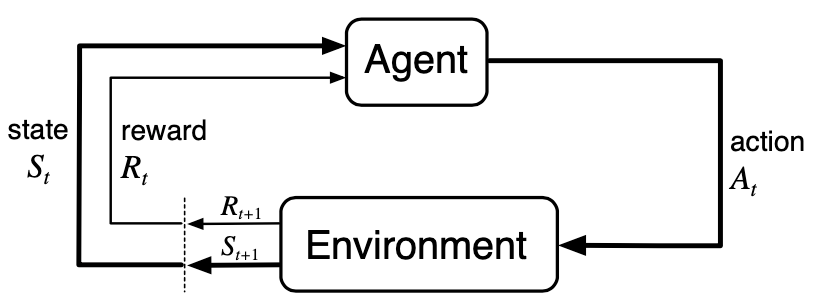
\includegraphics[width=0.65\linewidth]{images/RL.png}
\end{figure}
\end{frame}

\subsection{Q-learning}
\begin{frame}{Q-learning}
\begin{Definition}[Q-function]
	\[
	Q^\alpha(x,a) := r(x,a) + \gamma \mathbb E [v^\alpha(X_1^a)]
	\]
	\[
	Q^*(x,a) := r(x,a) + \gamma \mathbb E [v^*(X_1^a)]
	\]
\end{Definition}



From DPP, we know that, $\max_a Q^*(x,a) = v^*(x)$, therefore
\[
Q^*(x,a) = r(x,a) + \gamma \mathbb E^x [\max_{b\in A}Q^*(X^a_1,b)].
\]
Re-arranging, 
\[
0 = r(x,a) + \gamma \mathbb E^x [\max_{b\in A}Q^*(X^a_1,b)] - Q^*(x,a)
\]
\end{frame}

\begin{frame}{Q-learning Algorithm - Stochastic Approximation}
Stochastic approximation arises when one wants to find the root $\theta^*$ of the following expression
\[
0 = C(\theta) := \mathbb E_{X\sim \mu} (c(X,\theta))
\]
If we have access to unbiased approximations of $C(\theta)$, namely $\tilde C(\theta)$, then the following updates
\[
\theta \leftarrow \theta - \delta_n \tilde C(\theta) 
\]
 with $\delta_n\in(0,1)$ satisfying
\[
\sum_n \delta_n = +\infty, \quad \sum_n \delta_n^2 < +\infty
\]
will converge to $\theta^*$

Going back to Q-learning, we want to find an unbiased approximation of
\[
r(x,a) + \gamma \mathbb E^x [\max_{b\in A}Q^*(X^a_1,b)] - Q^*(x,a)
\]
%
%\begin{remark}[Stochastic Approximation]
%Note that $\max_{b\in A}Q(y,b)$ is an unbiased approx of $\mathbb E^x [\max_{b\in A}Q(X_1^a,b)]$. Hence we are doing stochastic approximation to find the root of  
%\[
%0 = f(a,x) + \gamma \mathbb E^x [\max_{b\in A}Q(X^a_1,b)] - Q(x,a)
%\]	
%\end{remark}
\end{frame}

\begin{frame}{Q-learning Algorithm}
Recall $\mathcal S, A$ are finite (they can be big). Transition probabilities, running cost and final cost are unknown, but we can observe tuples $(x_n, a_n, r_n,x_{n+1})$ from interacting with the environment. 
\begin{enumerate}
	\item Make initial guess, for $Q^*(x,a)$ denoted by $Q(x,a)$ for all $x,a$.
	\item We select and perform an action $a$ (either by following the current policy, or by doing some sort of exploration).
	\item We select the state we landed in, denoting it by $y$. If it is not terminal, adjust
	\[
	Q(x, a) \leftarrow Q(x, a) + \delta_n \left( r(x,a) + \gamma \max_{b\in A}Q(y,b) - Q(x,a)  \right)
	\]
	Note: we are doing Stochastic Approximation using $max_{b\in A}Q(y,b)$ as an unbiased approximation of $\mathbb E^x [\max_{b\in A}Q(X^a_1,b)]$.
	\item Go back to (2)
\end{enumerate}
\end{frame}



\begin{frame}{Q-learning Algorithm - Function approximation}
In practice, the state space might be very large (or continuous). It is then infeasible to sample $(x_n, a, r, x_{n+1})$ to explore all the space. 

Alternatively, $Q$ can be approximated with a Neural Network with parameters $\theta$. 

The optimal policy will be defined as $\alpha(x) = \max_{b\in A} Q_{\theta^*}(x,a)$ for some optimal parameters $\theta^*$.
\begin{enumerate}
\item Initialise network's parameters $\theta$.
\item Sample tuples $(x_n, a_n, r_n, x_{n+1})_{n=1,...,M}$ from the environment, using some exploration-exploitation heuristics. 
\item Find $\theta^*$ that minimise the $L_2$-error
\[
J(\theta) = \frac1{2}\, \mathbb E_{x,a\sim \mu} \left(Q_\theta(x,a) - (r(x,a) + \gamma \mathbb E^x \max_{b\in A} Q_{\bar \theta}(X,b)) \right)^2
\] 
where $\mu$ is the empirical measure of the visited  action-states,
using gradient ascent. We use the following approximation of the gradient
\[
\nabla_\theta J = \mathbb E_{x,a \sim \mu}\left(Q_\theta(x,a) - (r(x,a) + \gamma \mathbb E^x \max_{b\in A} Q_{\bar \theta}(X,b)) \right)\nabla_\theta Q_\theta(x,a)
\] 
\end{enumerate}
\end{frame}

\subsection{Policy Gradient}
\begin{frame}{Soft Policies}
From DPP it follows that the optimal policy is a deterministic function of the state. In practice, since the environment and the running cost/reward function are unkown, we will use \textbf{soft policies},
\[
\pi: \mathcal S \rightarrow \mathcal P(A)
\]
where $\mathcal P(A)$ is the space of probability meaures on $A$. 

I will abuse the notation, and I will indistinctively use  $\pi(\cdot | x)$ for the distribution, the probability mass function (or the density) of $\pi(x)$.

\begin{remark}[Relationship between the value function and the Q-function]
\[
v^\pi(x) = \mathbb E_{A\sim \pi(\cdot|x)} Q(x,A)
\]
\end{remark}


\end{frame}


\begin{frame}{Policy Gradient for Soft Policies I}
Consider a soft (random) policy with probability mass function $\pi_\theta(\cdot | x)$ parametrised by some parameters $\theta$. Let $\rho$ be some initial state distribution.  	
	
	Instead of finding the optimal policy through the Q-function, we directly maximise the expected return for all $x\in S$.
	\[
		J^{\pi_\theta}(\theta) = \mathbb E_{A_n\sim \pi(\cdot|X_n)} \left [ \sum_{n=0}^\infty \gamma^n r(A_n, X_n^\alpha) \bigg \vert X_0\sim \rho\right]
	\]
	
Assume we know an expression for $\nabla_\theta J^{\pi_\theta}$ (next slide). Then $\argmax_{\theta} J^{\pi_\theta}(\theta)$
is found using gradient ascent using a learning rate $\tau$
\[
\theta \leftarrow \theta + \tau \cdot \nabla_\theta J^{\pi_\theta}
\]
\end{frame}

\begin{frame}{Policy Gradient for Soft Policies II}
	 We need to find an expression for $\nabla_\theta J^{\pi_\theta}$. This is given by The Policy Gradient Thm, Section 13.2 in ~\cite{sutton2018reinforcement}
	\begin{Theorem}[Policy Gradient Theorem]
		\[
		\begin{split}
		\nabla_\theta J^{\pi_\theta}(\theta) &  \propto \sum_{x\in\mathcal S} \mu(x) \sum_{a\in A} \nabla_\theta \pi_\theta(a|x) Q_{\pi_\theta}(x,a)  \\ 
		 & \propto \mathbb E_{X_n\sim \mu} \left[ \mathbb E_{A_n\sim \pi_\theta(\cdot|X_n)} \nabla_\theta \log (\pi_\theta(A_n | X_n)) Q_{\pi_\theta}(X_n,A_n)\right]
		\end{split}
		\]
		where $\mu$ is the visitation measure. 
	\end{Theorem}
	\red{We need to approximate $Q_{\pi_\theta}$!}
\end{frame}


\begin{frame}{Policy Gradient for Deterministic Policies}
If we have a deterministic policy with continuous actions $\alpha_\alpha: \mathcal S \rightarrow A$, then the
Deterministic Policy Gradient for Reinforcement Learning with continuous actions is given by Theorem 1 in ~\cite{silver2014deterministic}
\begin{Theorem}
\[
\nabla_\theta J^{\alpha_\theta}(\theta) = \mathbb E_{X_n\sim \mu} \left[ \nabla_\theta \alpha_\theta(x) \nabla_a Q_{\alpha_\theta}(X_n, \alpha_\theta(s)) \right]
\]	
\end{Theorem}
\red{We need to approximate $Q_{\alpha_\theta}$}
\end{frame}


\begin{frame}{Actor-Critic type Algorithms}
Policy Gradient theorems include the Q-function. In practice, one can either 
\begin{itemize}
\item approximate it using Monte Carlo (i.e. by simulating several games starting from $(x,a)$ and approximate it with the average). This is expensive and might have a high variance. 
\item Using a function approximation $Q_\psi (x,a)$ with parameters $\psi$. This motivates \textbf{actor-critic} algorithms:

\begin{enumerate}
\item \textbf{Policy evaluation}: approximate the Q-function (the critic) using for example the Bellman equation.
\[
\psi^* = \argmax_{\psi}\frac1{2}\, \mathbb E_{x,a\sim \mu} \left(Q_\psi(x,a) - (r(x,a) + \gamma \mathbb E^x  v_{\bar \psi}(X)) \right)^2
\] 
where we recall that $v_{\bar \psi}(X) = \mathbb E_{a\sim \pi_\theta(\cdot|X)}[Q_\psi(X,a)] $
\item \textbf{Policy improvement} improve the policy (the actor) with gradient ascent using the Policy Gradient theorems. 
\end{enumerate}

\end{itemize}
\end{frame}




\begin{frame}[allowframebreaks]
\frametitle{References}

\bibliographystyle{apalike}
\bibliography{Bibliography} 
	
\end{frame}

\end{document}
